\chapter{लिगैंड क्षेत्र सिद्धांत और रंग}\label{ch:b2:ligand-field}

माणिक लाल है और पन्ना हरा, फिर भी दोनों अपना रंग एक ही आयन,
\ce{Cr^3+}, के कारण पाते हैं, जिसके कुछ आयन कोरंडम, \ce{Al2O3}, में या
बेरिल में ऐलुमिनियम का स्थान लेते हैं। कॉपर सल्फ़ेट के क्रिस्टल गहरे नीले होते हैं, परंतु उन्हें
गर्म करने के बाद बचा चूर्ण सफ़ेद होता है। हर स्थिति में रंग उन d कक्षकों के बीच
इलेक्ट्रॉनों की छलाँग से आता है जिनकी ऊर्जाओं को आसपास के परमाणुओं ने अलग-अलग खींच दिया है ---
उतना जितना इस पर निर्भर करता है कि आयन को कौन-से परमाणु और किस प्रकार घेरते हैं। यह
अध्याय उस विपाटन को परिकलित करता है, पहले बिंदु आवेशों से, फिर \omterm{def:b2:diatomic-mos:lcao}{आण्विक
कक्षकों} से; यह रंगों, चुंबकत्व, और पिछले अध्याय के \omterm{def:b2:coordination-complexes:electron-count}{18-इलेक्ट्रॉन नियम} की
व्याख्या करता है।

\begin{recall}
\Cref{ch:b2:coordination-complexes}: $d^n$ विन्यास, ज्यामितियाँ, इलेक्ट्रॉन
गणनाएँ। \Cref{ch:b2:atomic-orbitals}: पाँचों d कक्षकों की आकृतियाँ।
\Cref{ch:b2:fragment-orbitals}: \omterm{def:b2:fragment-orbitals:fragment}{अणुखंड कक्षक}। प्रथम वर्ष का खंड: अवशोषकता,
पूरक रंग, अयुग्मित इलेक्ट्रॉन, हुंड का नियम।
\end{recall}

\begin{omfigure}
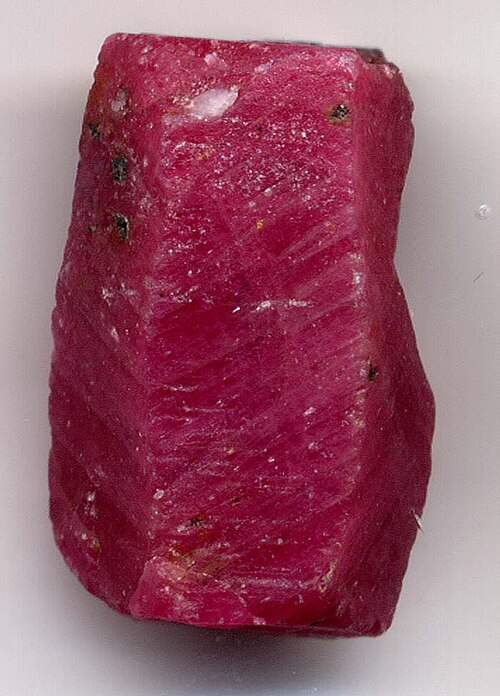
\includegraphics[height=3.6cm]{images/book3/ruby.jpg}\hspace{0.6cm}%
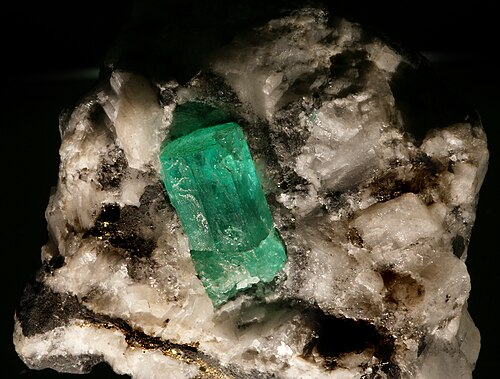
\includegraphics[height=3.6cm]{images/book3/emerald.jpg}\hspace{0.6cm}%
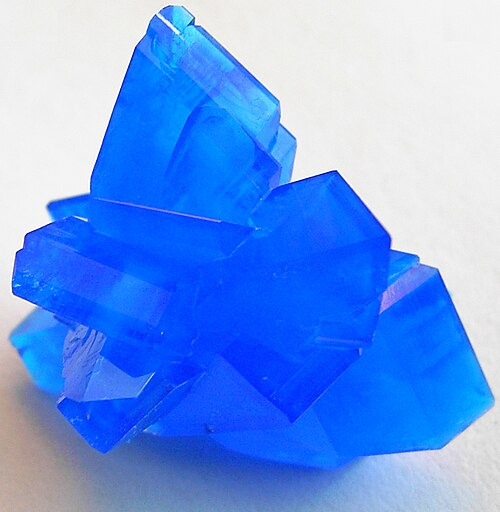
\includegraphics[height=3.6cm]{images/book3/copper-sulfate.jpg}

{\small माणिक का एक क्रिस्टल (सार्वजनिक अधिकार-क्षेत्र); अपनी चट्टान में एक पन्ना (दिदिए देकुअँ,
CC BY-SA 3.0); कॉपर(II) सल्फ़ेट पेंटाहाइड्रेट के क्रिस्टल (स्टेफ़ैनबी, CC BY-SA
3.0)। विकिमीडिया कॉमन्स। पहले दोनों को क्रोमियम(III) रंग देता है, तीसरे को
कॉपर(II) का ऐक्वा संकुल।}
\end{omfigure}

\section{क्रिस्टल-क्षेत्र मॉडल}

\begin{definition}[क्रिस्टल क्षेत्र]\label{def:b2:ligand-field:crystal-field}
\emph{क्रिस्टल-क्षेत्र मॉडल}\index{क्रिस्टल-क्षेत्र मॉडल} किसी संकुल के लिगैंडों को
धातु आयन के चारों ओर ऋणात्मक बिंदु आवेश (या द्विध्रुवों के ऋणात्मक सिरे) मानता है,
और परिकलित करता है कि वे उसके d कक्षकों की ऊर्जाओं को कैसे बदलते हैं। अष्टफलकीय
क्षेत्र में d कक्षक दो समुच्चयों में विपाटित होते हैं, जिनके बीच का अंतर \emph{क्रिस्टल-क्षेत्र
विपाटन}\index{क्रिस्टल-क्षेत्र विपाटन} $\Delta_o$ है।
\end{definition}

छह लिगैंडों को अक्षों पर रखिए। $\mathrm d_{z^2}$ और $\mathrm d_{x^2-y^2}$
कक्षक अपनी पालियाँ सीधे लिगैंडों की ओर करते हैं: उनमें स्थित इलेक्ट्रॉन अधिक प्रतिकर्षित होता है
और वे ऊपर उठते हैं। $\mathrm d_{xy}$, $\mathrm d_{xz}$, $\mathrm d_{yz}$ कक्षक
लिगैंडों के बीच इंगित करते हैं और कम उठते हैं। पहले युग्म को $e_g$ कहते हैं, तीन के दूसरे समुच्चय को
$t_{2g}$ (ये नाम समूह सिद्धांत से आते हैं, जो तृतीय वर्ष के खंड में है)।

\begin{omfigure}
\begin{tikzpicture}[font=\small]
  \begin{scope}
    \pic at (0,0) {omdx2y2};
    \foreach \p in {(1.25,0),(-1.25,0),(0,1.25),(0,-1.25)} \node[circle, fill=black!70, inner sep=2.2pt] at \p {};
    \node at (0,-1.75) {$\mathrm d_{x^2-y^2}$: पालियाँ लिगैंडों की ओर};
  \end{scope}
  \begin{scope}[xshift=5.5cm]
    \pic at (0,0) {omdxy};
    \foreach \p in {(1.25,0),(-1.25,0),(0,1.25),(0,-1.25)} \node[circle, fill=black!70, inner sep=2.2pt] at \p {};
    \node at (0,-1.75) {$\mathrm d_{xy}$: पालियाँ उनके बीच};
  \end{scope}
\end{tikzpicture}

{\small किसी अष्टफलक के $xy$ तल के चार लिगैंडों (काले बिंदु) के बीच दो d कक्षक।
$\mathrm d_{x^2-y^2}$ की पालियाँ लिगैंडों की ओर इंगित करती हैं,
$\mathrm d_{xy}$ की उनके बीच।}
\end{omfigure}

\begin{theorem}[भारकेंद्र]\label{thm:b2:ligand-field:barycentre}
अष्टफलकीय क्षेत्र में, d कक्षकों की औसत ऊर्जा से मापने पर,
$e_g$ युग्म $+0.6\Delta_o$ पर और $t_{2g}$ समुच्चय $-0.4\Delta_o$ पर होता है।
\end{theorem}

\begin{proof}
क्षेत्र पाँचों d ऊर्जाओं के औसत को ऊपर उठाता है, परंतु विपाटन से उसे नहीं बदलता
(भारकेंद्र नियम, स्वीकृत: कक्षकों के किसी पूर्ण समुच्चय के विस्थापनों का योग
कुल आवेश से निर्धारित होता है, उसकी व्यवस्था से नहीं)। $e_g$ को $x$ पर और
$t_{2g}$ को $x - \Delta_o$ पर रखने पर प्रतिबंध $2x + 3(x - \Delta_o) = 0$ से $x = 0.6\Delta_o$ मिलता है।
\end{proof}

\section{उच्च चक्रण और निम्न चक्रण}

\begin{definition}[चक्रण अवस्थाएँ]\label{def:b2:ligand-field:spin}
\emph{युग्मन ऊर्जा}\index{युग्मन ऊर्जा} $P$ वह ऊर्जा है जो किसी दूसरे
इलेक्ट्रॉन को समान ऊर्जा के किसी खाली कक्षक के स्थान पर किसी भरे कक्षक में रखने के लिए चाहिए। कोई
संकुल \emph{उच्च चक्रण}\index{उच्च चक्रण} वाला है जब उसके इलेक्ट्रॉन $e_g$ कक्षकों में जाते हैं,
$t_{2g}$ में युग्मित होने से पहले, और \emph{निम्न चक्रण}\index{निम्न चक्रण} वाला जब वे पहले
$t_{2g}$ में युग्मित होते हैं।
\end{definition}

\begin{proposition}[चक्रण अवस्था का चयन]\label{prop:b2:ligand-field:spin-state}
$d^4$ से $d^7$ तक के अष्टफलकीय आयनों के लिए संकुल \omterm{def:b2:ligand-field:spin}{निम्न चक्रण} वाला है यदि $\Delta_o > P$, और \omterm{def:b2:ligand-field:spin}{उच्च चक्रण} वाला
यदि $\Delta_o < P$। $d^1$--$d^3$ और $d^8$--$d^{10}$ के लिए केवल एक विन्यास होता है।
\end{proposition}

\begin{proof}
$d^3$ ($t_{2g}^3$) से आगे चौथा इलेक्ट्रॉन या तो $e_g$ में जाता है (लागत $\Delta_o$,
$t_{2g}$ से ऊपर) या $t_{2g}$ में युग्मित होता है (लागत $P$)। सस्ता विकल्प जीतता है; यही तुलना
$d^7$ तक हर इलेक्ट्रॉन पर लागू होती है। $d^1$--$d^3$ के लिए $t_{2g}$ में बिना युग्मन के स्थान है;
$d^8$--$d^{10}$ के लिए $t_{2g}$ भरा है और $e_g$ का उपयोग वैसे भी करना पड़ता है।
\end{proof}

\begin{definition}[क्रिस्टल-क्षेत्र स्थायीकरण ऊर्जा]\label{def:b2:ligand-field:cfse}
किसी विन्यास $t_{2g}^ae_g^b$ की \emph{क्रिस्टल-क्षेत्र स्थायीकरण ऊर्जा}\index{क्रिस्टल-क्षेत्र स्थायीकरण ऊर्जा}
(CFSE) $(-0.4a + 0.6b)\Delta_o$ है, अर्थात् भारकेंद्र के सापेक्ष
d इलेक्ट्रॉनों की ऊर्जा (युग्मन ऊर्जाएँ अलग से गिनी जाती हैं)।
\end{definition}

\begin{proposition}[श्रेणी के अनुदिश CFSE]\label{prop:b2:ligand-field:cfse}
\omterm{def:b2:ligand-field:spin}{उच्च चक्रण} में CFSE $0$, $-0.4$, $-0.8$, $-1.2$, $-0.6$, $0$, $-0.4$, $-0.8$, $-1.2$,
$-0.6$, $0$ ($\Delta_o$ में) है, $d^0$ से $d^{10}$ तक: यह $d^0$, $d^5$, $d^{10}$ के लिए शून्य होती है। \omterm{def:b2:ligand-field:spin}{निम्न
चक्रण} में यह $-2.4\Delta_o$ तक पहुँचती है, $d^6$ के लिए।
\end{proposition}

\begin{proof}
विन्यासों को भरिए और परिभाषा लागू कीजिए; मान वही हैं जो चित्र में हैं,
परिकलित।
\end{proof}

\begin{omfigure}
\begin{tikzpicture}
\begin{axis}[width=0.55\linewidth, height=5cm, xmin=-0.5, xmax=10.5, ymin=-2.6, ymax=0.3,
  axis x line=bottom, axis y line=left, xlabel={$d^n$}, ylabel={CFSE ($\Delta_o$)},
  xtick={0,1,2,3,4,5,6,7,8,9,10}, tick label style={font=\small}, label style={font=\small}]
\addplot[omThm, thick, mark=*, mark size=1.3pt] table[x=n, y=high] {figdata/out/bachelor-2-ligand-field-a.dat};
\addplot[omDef, thick, dashed, mark=square*, mark size=1.3pt] table[x=n, y=low] {figdata/out/bachelor-2-ligand-field-a.dat};
\node[font=\scriptsize, omThm, anchor=west] at (axis cs:5.4,0.0) {उच्च चक्रण};
\node[font=\scriptsize, omDef, anchor=west] at (axis cs:6.6,-2.2) {निम्न चक्रण};
\end{axis}
\end{tikzpicture}\hfill
\begin{tikzpicture}[font=\small]
  \pic (t) at (0,0) {omlevel={ud}{0.5}}; \pic at (0.6,0) {omlevel={u}{0.5}}; \pic at (1.2,0) {omlevel={u}{0.5}};
  \pic at (0.3,1.6) {omlevel={u}{0.5}}; \pic at (0.9,1.6) {omlevel={u}{0.5}};
  \node at (0.6,-0.8) {उच्च चक्रण $d^6$};
  \node[font=\scriptsize, anchor=east] at (-0.35,0) {$t_{2g}$}; \node[font=\scriptsize, anchor=east] at (-0.05,1.6) {$e_g$};
  \pic at (3,0) {omlevel={ud}{0.5}}; \pic at (3.6,0) {omlevel={ud}{0.5}}; \pic at (4.2,0) {omlevel={ud}{0.5}};
  \pic at (3.3,2.4) {omlevel={empty}{0.5}}; \pic at (3.9,2.4) {omlevel={empty}{0.5}};
  \node at (3.6,-0.8) {निम्न चक्रण $d^6$};
  \draw[<->, omProp] (4.7,0) -- (4.7,2.4) node[midway, right, font=\scriptsize] {$\Delta_o$};
  \draw[<->, omProp] (1.7,0) -- (1.7,1.6) node[midway, right, font=\scriptsize] {$\Delta_o$};
\end{tikzpicture}

{\small बाएँ: d श्रेणी के अनुदिश \omterm{def:b2:ligand-field:cfse}{क्रिस्टल-क्षेत्र स्थायीकरण ऊर्जा} (परिकलित),
\omterm{def:b2:ligand-field:spin}{उच्च चक्रण} (ठोस) और \omterm{def:b2:ligand-field:spin}{निम्न चक्रण} (खंडित)। दाएँ: किसी $d^6$
आयन के दो विन्यास: $\Delta_o < P$ होने पर चार अयुग्मित इलेक्ट्रॉन (जैसे \ce{[Fe(H2O)6]^2+}), $\Delta_o >
P$ होने पर एक भी नहीं (जैसे \ce{[Fe(CN)6]^4-})।}
\end{omfigure}

\begin{method}[चक्रण अवस्था, CFSE और अयुग्मित इलेक्ट्रॉन]\label{met:b2:ligand-field:spin-state}
\begin{enumerate}
  \item ऑक्सीकरण अवस्था से $n$ ज्ञात कीजिए ($n = g - m$)।
  \item $d^4$--$d^7$ के लिए $\Delta_o$ और $P$ की तुलना कीजिए (या लिगैंड को
        \omterm{def:b2:ligand-field:spectrochemical}{स्पेक्ट्रमरासायनिक श्रेणी} में रखिए): प्रबल क्षेत्र, \omterm{def:b2:ligand-field:spin}{निम्न चक्रण}; दुर्बल क्षेत्र, \omterm{def:b2:ligand-field:spin}{उच्च चक्रण}।
  \item उसी के अनुसार $t_{2g}$ और $e_g$ भरिए; CFSE $= (-0.4a + 0.6b)\Delta_o$।
  \item अयुग्मित इलेक्ट्रॉन गिनिए; कोई भी अयुग्मित इलेक्ट्रॉन संकुल को
        \omterm{def:b2:diatomic-mos:magnetism}{अनुचुंबकीय} बनाता है।
\end{enumerate}
\end{method}

\section{अन्य ज्यामितियाँ}

\begin{proposition}[चतुष्फलकीय और वर्ग समतलीय क्षेत्र]\label{prop:b2:ligand-field:tetrahedral}
चतुष्फलकीय क्षेत्र में क्रम उलट जाता है: दो कक्षक ($e$) तीन ($t_2$) के नीचे,
उसी धातु और उन्हीं लिगैंडों के लिए विपाटन $\Delta_t \approx \frac49\Delta_o$ के साथ; चतुष्फलकीय
संकुल \omterm{def:b2:ligand-field:spin}{उच्च चक्रण} वाले होते हैं। वर्ग समतलीय क्षेत्र में $\mathrm d_{x^2-y^2}$ कक्षक अन्य कक्षकों से बहुत
ऊपर होता है: कोई $d^8$ आयन चारों निचले कक्षकों को भरता है और उसे खाली छोड़ देता है।
\end{proposition}

\admitted

गुणक $4/9$ बिंदु आवेशों की ज्यामिति से आता है; केवल चार लिगैंडों के साथ,
जिनमें से कोई अक्षों के अनुदिश इंगित नहीं करता, विपाटन \omterm{def:b2:ligand-field:spin}{युग्मन ऊर्जा}
से पार पाने के लिए बहुत छोटा है। किसी अष्टफलक के $z$ अक्ष के दोनों लिगैंडों को हटाने से
$z$ घटक वाले कक्षक नीचे आते हैं और कुछ भी ऊपर नहीं उठता: इससे
पिछले अध्याय के वर्ग समतलीय $d^8$ संकुलों की व्याख्या होती है, जिनके आठों इलेक्ट्रॉन खाली
$\mathrm d_{x^2-y^2}$ के नीचे स्थान पा जाते हैं।

\begin{omfigure}
\begin{tikzpicture}[font=\scriptsize]
  % octahedral
  \pic at (-0.3,0) {omlevel={empty}{0.45}}; \pic at (0.25,0) {omlevel={empty}{0.45}}; \pic at (0.8,0) {omlevel={empty}{0.45}};
  \pic at (0,1.8) {omlevel={empty}{0.45}}; \pic at (0.55,1.8) {omlevel={empty}{0.45}};
  \node[anchor=west] at (1.1,0) {$t_{2g}$}; \node[anchor=west] at (0.85,1.8) {$e_g$};
  \node[font=\small] at (0.25,-0.7) {अष्टफलकीय};
  % tetrahedral
  \begin{scope}[xshift=3.5cm]
    \pic at (0,0.6) {omlevel={empty}{0.45}}; \pic at (0.55,0.6) {omlevel={empty}{0.45}};
    \pic at (-0.3,1.4) {omlevel={empty}{0.45}}; \pic at (0.25,1.4) {omlevel={empty}{0.45}}; \pic at (0.8,1.4) {omlevel={empty}{0.45}};
    \node[anchor=west] at (0.85,0.6) {$e$}; \node[anchor=west] at (1.1,1.4) {$t_2$};
    \node[font=\small] at (0.25,-0.7) {चतुष्फलकीय};
  \end{scope}
  % square planar
  \begin{scope}[xshift=7cm]
    \pic at (0,-0.2) {omlevel={empty}{0.45}}; \pic at (0.55,-0.2) {omlevel={empty}{0.45}};
    \pic at (0.25,0.3) {omlevel={empty}{0.45}};
    \pic at (0.25,0.9) {omlevel={empty}{0.45}};
    \pic at (0.25,2.6) {omlevel={empty}{0.45}};
    \node[anchor=west] at (0.85,-0.2) {$\mathrm d_{xz}, \mathrm d_{yz}$};
    \node[anchor=west] at (0.55,0.3) {$\mathrm d_{z^2}$};
    \node[anchor=west] at (0.55,0.9) {$\mathrm d_{xy}$};
    \node[anchor=west] at (0.55,2.6) {$\mathrm d_{x^2-y^2}$};
    \node[font=\small] at (0.25,-0.7) {वर्ग समतलीय};
  \end{scope}
\end{tikzpicture}

{\small तीन ज्यामितियों में d कक्षकों का विपाटन, व्यवस्था-रूप (एक ही पैमाने पर
नहीं): अष्टफलकीय, चतुष्फलकीय (उलटा और छोटा), वर्ग समतलीय (एक कक्षक अन्य कक्षकों से बहुत
ऊपर)।}
\end{omfigure}

\section{रंग और स्पेक्ट्रमरासायनिक श्रेणी}

\begin{definition}[d–d संक्रमण]\label{def:b2:ligand-field:d-d}
\emph{d–d संक्रमण}\index{d–d संक्रमण} प्रकाश के अवशोषण द्वारा किसी संकुल के
निचले से ऊँचे d स्तर पर किसी इलेक्ट्रॉन का उन्नयन है; किसी $d^1$ आयन के लिए
$t_{2g}$ से $e_g$ तक, ऊर्जा $\Delta_o$ पर।
\end{definition}

\begin{proposition}[रंग से विपाटन]\label{prop:b2:ligand-field:colour}
यदि कोई संकुल तरंगदैर्ध्य $\lambda_{\max}$ पर ऊर्जा $\Delta_o$ के किसी \omterm{def:b2:ligand-field:d-d}{d–d संक्रमण} से
सबसे प्रबल अवशोषण करता है, तो प्रति मोल $\Delta_o = N_Ahc/\lambda_{\max}$, या तरंग संख्याओं में $\tilde\nu = 1/\lambda_{\max}$;
दिखने वाला रंग अवशोषित रंग का पूरक होता है।
\end{proposition}

\begin{proof}
तरंगदैर्ध्य $\lambda$ का फ़ोटॉन $hc/\lambda$ वहन करता है; फ़ोटॉनों का एक मोल, $N_Ahc/\lambda$। श्वेत
प्रकाश में से अवशोषित पट्टी घटा देने पर पूरक रंग दिखता है।
\end{proof}

\begin{method}[अवशोषण पट्टी से रंग तक]\label{met:b2:ligand-field:colour}
\begin{enumerate}
  \item $\lambda_{\max}$ को $\tilde\nu = 1/\lambda_{\max}$ (\unit{cm^{-1}}) और
        $N_Ahc/\lambda_{\max}$ (\unit{kJ/mol}) में बदलिए: $\qty{500}{nm} \leftrightarrow \qty{20000}{cm^{-1}}
        \leftrightarrow \qty{239}{kJ/mol}$।
  \item अवशोषित रंग ज्ञात कीजिए (बैंगनी 400--430, नीला 430--490, हरा 490--560, पीला
        560--590, नारंगी 590--620, लाल 620--700 nm, लगभग)।
  \item दिखने वाला रंग रंग-चक्र पर सामने वाला रंग है।
\end{enumerate}
\end{method}

\begin{omfigure}
\begin{tikzpicture}[font=\scriptsize]
  \foreach \a/\c/\n in {90/red/लाल, 150/orange/नारंगी, 210/yellow/पीला, 270/green!70!black/हरा, 330/blue/नीला, 30/violet/बैंगनी} {
    \fill[\c!75] (0,0) -- (\a-30:1.3) arc[start angle=\a-30, end angle=\a+30, radius=1.3] -- cycle;
    \node[anchor=\a+180] at (\a:1.38) {\n};
  }
  \draw[thick] (0,0) circle (1.3);
  \draw[<->, thick] (90:0.9) -- (270:0.9);
  \node[anchor=west, font=\small, align=left] at (2.6,0) {हरा अवशोषित हो (लगभग 500--560 nm)\\ तो संकुल लाल-बैंगनी दिखता है;\\ नारंगी अवशोषित हो तो नीला।};
\end{tikzpicture}

{\small एक रंग-चक्र: दिखने वाला रंग मोटे तौर पर अवशोषित पट्टी का पूरक होता है, जो
व्यासतः सामने होता है।}
\end{omfigure}

\begin{definition}[स्पेक्ट्रमरासायनिक श्रेणी]\label{def:b2:ligand-field:spectrochemical}
\emph{स्पेक्ट्रमरासायनिक श्रेणी}\index{स्पेक्ट्रमरासायनिक श्रेणी} लिगैंडों को किसी दिए गए
धातु आयन के लिए उनके द्वारा उत्पन्न विपाटन के क्रम में रखती है:
\[
  \ce{I-} < \ce{Br-} < \ce{Cl-} < \ce{F-} < \ce{OH-} < \ce{H2O} < \ce{NH3} < \text{en} <
  \ce{NO2-} < \ce{CN-} < \ce{CO} .
\]
किसी दिए गए लिगैंड के लिए $\Delta_o$ धातु आयन के आवेश के साथ और समूह में नीचे जाने पर भी बढ़ता है
(4d और 5d संकुल, जो 3d से बड़े हैं, लगभग सदैव \omterm{def:b2:ligand-field:spin}{निम्न चक्रण} वाले होते हैं)।
\end{definition}

हैलाइड दुर्बल सिरे पर हैं और \ce{CN-} तथा \ce{CO} प्रबल सिरे पर, जिसकी
\omterm{def:b2:ligand-field:crystal-field}{क्रिस्टल-क्षेत्र मॉडल} व्याख्या नहीं कर सकता: वह आवेशित \ce{F-} को उदासीन
\ce{CO} से ऊपर रखता। व्याख्या के लिए कक्षक चाहिए।

\section{लिगैंड क्षेत्र}

\begin{definition}[लिगैंड क्षेत्र सिद्धांत]\label{def:b2:ligand-field:ligand-field}
\emph{लिगैंड क्षेत्र सिद्धांत}\index{लिगैंड क्षेत्र सिद्धांत} किसी संकुल का वर्णन उन \omterm{def:b2:diatomic-mos:lcao}{आण्विक कक्षकों} से करता है
जो धातु के संयोजकता कक्षकों (उसके नौ $n$d, $(n+1)$s और $(n+1)$p
कक्षकों) और लिगैंडों के दाता कक्षकों से बने हों।
\end{definition}

\begin{proposition}[अष्टफलकीय संकुल में $\sigma$ आबंधन]\label{prop:b2:ligand-field:mo-octahedral}
छह लिगैंडों के साथ, जिनमें से हर एक एक $\sigma$ दाता कक्षक देता है, छह आबंधी \omterm{def:b2:diatomic-mos:lcao}{आण्विक कक्षक}
धातु के s, तीनों p और दोनों $e_g$ d कक्षकों से बनते हैं; तीनों $t_{2g}$ कक्षक, जो
लिगैंडों के बीच इंगित करते हैं, अनाबंधी रहते हैं; उनके ऊपर प्रतिआबंधी $e_g^*$
कक्षक होते हैं। लिगैंडों के इलेक्ट्रॉन छहों \omterm{def:b2:diatomic-mos:bonding}{आबंधी कक्षकों} को भरते हैं; धातु के d इलेक्ट्रॉन
$t_{2g}$ और $e_g^*$ में जाते हैं, जो $\Delta_o$ से अलग हैं। आबंधी और \omterm{def:b2:diatomic-mos:bonding}{अनाबंधी कक्षक} मिलकर
$12 + 6 = 18$ इलेक्ट्रॉन रख सकते हैं।
\end{proposition}

\begin{proof}[तर्क]
\cref{ch:b2:fragment-orbitals} की \omterm{def:b2:fragment-orbitals:fragment}{अणुखंड} विधि से धातु का हर कक्षक
लिगैंड कक्षकों के उसी सममिति वाले संयोजन से अन्योन्यक्रिया करता है: s पूर्णतः
सममित संयोजन से, हर p आमने-सामने के लिगैंडों के एक युग्म से, $\mathrm d_{z^2}$ और $\mathrm
d_{x^2-y^2}$ अपनी पालियों के अनुदिश इंगित करने वाले संयोजनों से; कोई $\sigma$ संयोजन
$t_{2g}$ कक्षकों से मेल नहीं खाता (किसी अक्ष के अनुदिश इंगित करने वाले किसी भी $\sigma$ दाता से उनका अतिव्यापन
सममिति से शून्य है)। संयोजनों के नाम समूह सिद्धांत से आते हैं, स्वीकृत।
सभी आबंधी और \omterm{def:b2:diatomic-mos:bonding}{अनाबंधी कक्षकों} को भरने, और किसी प्रतिआबंधी को नहीं, में
18 इलेक्ट्रॉन लगते हैं --- \omterm{def:b2:coordination-complexes:electron-count}{18-इलेक्ट्रॉन नियम}।
\end{proof}

\begin{omfigure}
\begin{tikzpicture}[font=\scriptsize]
  % metal
  \pic (m4p1) at (-0.45,2.6) {omlevel={empty}{0.4}}; \pic (m4p2) at (0,2.6) {omlevel={empty}{0.4}}; \pic (m4p3) at (0.45,2.6) {omlevel={empty}{0.4}};
  \node[anchor=east] at (-0.7,2.6) {$(n{+}1)$p};
  \pic (m4s) at (0,1.8) {omlevel={empty}{0.6}}; \node[anchor=east] at (-0.35,1.8) {$(n{+}1)$s};
  \foreach \x in {-0.9,-0.45,0,0.45,0.9} \pic at (\x,0.6) {omlevel={empty}{0.4}};
  \coordinate (m3d) at (1.1,0.6); \node[anchor=east] at (-1.15,0.6) {$n$d};
  \node[font=\small] at (0,-2.9) {धातु};
  % ligands
  \foreach \x in {6.2,6.72,7.24,7.76,8.28,8.8} \pic at (\x,-0.9) {omlevel={ud}{0.36}};
  \coordinate (lig) at (6.0,-0.9);
  \node[font=\small] at (7.3,-2.9) {छह $\sigma$ दाता कक्षक};
  % MOs
  \pic (b1) at (3.6,-2.4) {omlevel={ud}{0.5}};
  \foreach \x in {3.0,3.6,4.2} \pic at (\x,-1.9) {omlevel={ud}{0.5}};
  \pic at (3.3,-1.45) {omlevel={ud}{0.5}}; \pic at (3.9,-1.45) {omlevel={ud}{0.5}};
  \foreach \x in {3.0,3.6,4.2} \pic at (\x,0.3) {omlevel={empty}{0.5}};
  \pic at (3.3,1.5) {omlevel={empty}{0.5}}; \pic at (3.9,1.5) {omlevel={empty}{0.5}};
  \pic at (3.6,3.1) {omlevel={empty}{0.5}};
  \foreach \x in {3.0,3.6,4.2} \pic at (\x,3.6) {omlevel={empty}{0.5}};
  \node[anchor=north] at (3.6,0.12) {$t_{2g}$ (अनाबंधी)};
  \node[anchor=west] at (4.2,1.5) {$e_g^*$};
  \node[anchor=north] at (3.6,-2.58) {6 आबंधी};
  \draw[<->, omProp] (2.55,0.3) -- (2.55,1.5) node[midway, right] {$\Delta_o$};
  \draw[omcorr, densely dashed] (m3d) -- (2.75,0.3) (m3d) -- (3.05,1.5) (1.1,0.6) -- (3.05,-1.45);
  \draw[omcorr, densely dashed] (lig) -- (4.15,-1.45) (lig) -- (4.45,-1.9) (lig) -- (3.85,-2.4) (lig) -- (4.15,1.5);
  \draw[omcorr, densely dashed] (m4s-r) -- (3.35,-2.4) (m4s-r) -- (3.35,3.1) (m4p3-r) -- (2.75,-1.9) (m4p3-r) -- (2.75,3.6);
\end{tikzpicture}

{\small छह $\sigma$ दाताओं वाले किसी अष्टफलकीय संकुल के \omterm{def:b2:diatomic-mos:lcao}{आण्विक कक्षक},
व्यवस्था-रूप। लिगैंडों के बारह इलेक्ट्रॉन छहों \omterm{def:b2:diatomic-mos:bonding}{आबंधी कक्षकों} को भरते हैं; धातु के d
इलेक्ट्रॉन अनाबंधी $t_{2g}$ और प्रतिआबंधी $e_g^*$ स्तरों में रहते हैं, जो
$\Delta_o$ से अलग हैं --- क्रिस्टल-क्षेत्र चित्र फिर से प्राप्त। अधिकतम 18 इलेक्ट्रॉन आबंधी और
अनाबंधी स्तरों को भरते हैं।}
\end{omfigure}

\begin{definition}[$\pi$-दाता और $\pi$-ग्राही लिगैंड]\label{def:b2:ligand-field:pi-ligands}
\emph{$\pi$-दाता लिगैंड}\index{पाई-दाता लिगैंड@$\pi$-दाता लिगैंड} के पास धातु--लिगैंड आबंध
के सापेक्ष $\pi$ सममिति के भरे कक्षक होते हैं (\ce{Cl-},
\ce{OH-} के एकाकी युग्म); \emph{$\pi$-ग्राही लिगैंड}\index{पाई-ग्राही लिगैंड@$\pi$-ग्राही लिगैंड}
के पास निम्न ऊर्जा के खाली कक्षक होते हैं (\ce{CO} और \ce{CN-} के $\pi^*$ कक्षक)। भरे धातु d कक्षकों से
खाली $\pi^*$ कक्षकों में, जो किसी $\pi$-ग्राही लिगैंड के हों, इलेक्ट्रॉन घनत्व के
स्थानांतरण को \emph{पश्च-दान}\index{पश्च-दान} कहते हैं।
\end{definition}

\begin{proposition}[विपाटन पर $\pi$ प्रभाव]\label{prop:b2:ligand-field:pi-effects}
$\pi$-दाता लिगैंड $\Delta_o$ को घटाते हैं; $\pi$-ग्राही लिगैंड उसे बढ़ाते हैं।
\end{proposition}

\begin{proof}
$t_{2g}$ कक्षकों की सममिति लिगैंड $\pi$ कक्षकों से अतिव्यापन के लिए उपयुक्त है। भरा
लिगैंड $\pi$ कक्षक $t_{2g}$ से नीचे होता है: \cref{thm:b2:frontier-orbitals:perturbation} से
अन्योन्यक्रिया $t_{2g}$ को ऊपर, $e_g^*$ की ओर, धकेलती है, और $\Delta_o$ सिकुड़ता है। खाली $\pi^*$ कक्षक
$t_{2g}$ से ऊपर होता है: अन्योन्यक्रिया $t_{2g}$ को नीचे धकेलती है, और $\Delta_o$ बढ़ता है। दूसरी स्थिति
धातु का d घनत्व लिगैंड के $\pi^*$ में स्थानांतरित करती है: \omterm{def:b2:ligand-field:pi-ligands}{पश्च-दान}।
\end{proof}

\begin{omfigure}
\begin{tikzpicture}[font=\scriptsize]
  \begin{scope}
    \pic (t) at (0,1.2) {omlevel={empty}{0.6}}; \node[anchor=east] at (-0.35,1.2) {$t_{2g}$};
    \pic (l) at (2.4,0) {omlevel={ud}{0.6}}; \node[anchor=west] at (2.75,0) {लिगैंड $\pi$ (भरा)};
    \pic (n) at (1.2,1.75) {omlevel={empty}{0.6}};
    \draw[omcorr, densely dashed] (t-r) -- (n-l) (l-l) -- (n-r);
    \pic (e) at (1.2,3.0) {omlevel={empty}{0.6}}; \node[anchor=west] at (1.55,3.0) {$e_g^*$};
    \draw[<->, omProp] (0.55,1.75) -- (0.55,3.0) node[midway, left] {$\Delta_o$ छोटा};
    \node[font=\small] at (1.2,-0.8) {$\pi$ दाता};
  \end{scope}
  \begin{scope}[xshift=6.5cm]
    \pic (t) at (0,1.2) {omlevel={empty}{0.6}}; \node[anchor=east] at (-0.35,1.2) {$t_{2g}$};
    \pic (l) at (2.4,2.6) {omlevel={empty}{0.6}}; \node[anchor=west] at (2.75,2.6) {लिगैंड $\pi^*$ (खाली)};
    \pic (n) at (1.2,0.65) {omlevel={empty}{0.6}};
    \draw[omcorr, densely dashed] (t-r) -- (n-l) (l-l) -- (n-r);
    \pic (e) at (1.2,3.0) {omlevel={empty}{0.6}}; \node[anchor=west] at (1.55,3.15) {$e_g^*$};
    \draw[<->, omProp] (0.55,0.65) -- (0.55,3.0) node[midway, left] {$\Delta_o$ बड़ा};
    \node[font=\small] at (1.2,-0.8) {$\pi$ ग्राही (पश्च-दान)};
  \end{scope}
\end{tikzpicture}

{\small लिगैंड $\pi$ कक्षकों का $t_{2g}$ स्तर पर प्रभाव, व्यवस्था-रूप। नीचे स्थित भरा लिगैंड $\pi$
कक्षक $t_{2g}$ को ऊपर धकेलता है (छोटा विपाटन); ऊपर स्थित खाली $\pi^*$ कक्षक उसे नीचे
खींचता है (बड़ा विपाटन)।}
\end{omfigure}

इससे \ce{CO} और \ce{CN-}, जो प्रबल $\sigma$ दाता और $\pi$ ग्राही हैं, \omterm{def:b2:ligand-field:spectrochemical}{स्पेक्ट्रमरासायनिक श्रेणी} के
शीर्ष पर आते हैं, और हैलाइड, जो $\pi$ दाता हैं, तल पर। धातु कार्बोनिलों के
$t_{2g}$ कक्षक स्थायीकृत और भरे होते हैं: \cref{ch:b2:coordination-complexes} के
18-इलेक्ट्रॉन संकुल।

\section{अभ्यास}

\begin{exercise}[$\star$]\label{exo:b2:ligand-field:1}
किसी $d^3$ आयन और किसी $d^8$ आयन का अष्टफलकीय विन्यास और CFSE दीजिए।
\end{exercise}

\begin{exercise}[$\star$]\label{exo:b2:ligand-field:2}
\ce{[Fe(H2O)6]^2+} (\omterm{def:b2:ligand-field:spin}{उच्च चक्रण}) और \ce{[Fe(CN)6]^4-} (\omterm{def:b2:ligand-field:spin}{निम्न
चक्रण}) के कितने अयुग्मित इलेक्ट्रॉन हैं?
\end{exercise}

\begin{exercise}[$\star$]\label{exo:b2:ligand-field:3}
कोई संकुल \qty{600}{nm} पर सबसे प्रबल अवशोषण करता है। वह किस रंग का दिखता है?
\end{exercise}

\begin{exercise}[$\star$]\label{exo:b2:ligand-field:4}
\ce{H2O}, \ce{CN-}, \ce{Cl-}, \ce{NH3} को उनके द्वारा उत्पन्न विपाटन के क्रम में रखिए।
\end{exercise}

\begin{exercise}[$\star\star$]\label{exo:b2:ligand-field:5}
किसी $d^5$ आयन के लिए जल के साथ $\Delta_o = \qty{165}{kJ/mol}$ और सायनाइड के साथ $\qty{390}{kJ/mol}$ है,
और $P = \qty{300}{kJ/mol}$ (अभ्यास के आँकड़े)। दोनों चक्रण अवस्थाओं और अयुग्मित
इलेक्ट्रॉनों का पूर्वानुमान कीजिए।
\end{exercise}

\begin{exercise}[$\star\star$]\label{exo:b2:ligand-field:6}
\ce{[Co(H2O)6]^2+} गुलाबी है, \ce{[CoCl4]^2-} गहरा नीला। रंग के परिवर्तन को
ज्यामिति और लिगैंड के परिवर्तन से समझाइए।
\end{exercise}

\begin{exercise}[$\star\star$]\label{exo:b2:ligand-field:7}
दिखाइए कि वर्ग समतलीय \ce{[Ni(CN)4]^2-} \omterm{def:b2:diatomic-mos:magnetism}{प्रतिचुंबकीय} है, जबकि चतुष्फलकीय
\ce{[NiCl4]^2-} के दो अयुग्मित इलेक्ट्रॉन हैं।
\end{exercise}

\begin{exercise}[$\star\star$]\label{exo:b2:ligand-field:8}
कोई $d^1$ संकुल \qty{500}{nm} पर अवशोषण करता है (अभ्यास के आँकड़े)। $\Delta_o$ को \unit{cm^{-1}} और
\unit{kJ/mol} में परिकलित कीजिए।
\end{exercise}

\begin{exercise}[$\star\star$]\label{exo:b2:ligand-field:9}
\ce{Zn^2+} और \ce{Sc^3+} के यौगिक रंगहीन क्यों होते हैं?
\end{exercise}

\begin{exercise}[$\star\star\star$]\label{exo:b2:ligand-field:10}
\ce{[Co(NH3)6]^3+} के \omterm{def:b2:diatomic-mos:lcao}{आण्विक कक्षकों} में इलेक्ट्रॉन गिनिए: कौन-से स्तर भरे हैं,
और क्या संकुल \omterm{def:b2:diatomic-mos:magnetism}{प्रतिचुंबकीय} है?
\end{exercise}

\begin{exercise}[$\star\star\star$]\label{exo:b2:ligand-field:11}
समझाइए कि \ce{CO}, एक उदासीन और दुर्बल क्षारकीय अणु, फ़्लुओराइड आयन की तुलना में
बड़ा विपाटन क्यों उत्पन्न करता है।
\end{exercise}

\begin{exercise}[$\star\star\star$]\label{exo:b2:ligand-field:12}
\ce{M^2+} आयनों की, \ce{Ca^2+} से \ce{Zn^2+} तक, जलयोजन एन्थैल्पियाँ $n$ के विरुद्ध आलेखित करने पर
$d^0$, $d^5$ और $d^{10}$ से होकर जाने वाली सरल रेखा के ऊपर दो कूबड़ बनाती हैं। उच्च-चक्रण CFSE से
आकृति को समझाइए।
\end{exercise}

\section{समस्या: लाल माणिक, हरा पन्ना}

\begin{problem}[{सप्ताहांत समस्या --- अष्टफलकीय क्षेत्र में क्रोमियम(III), माणिक की अवशोषण
पट्टियाँ और वे जो रंग छोड़ती हैं, पन्ने का दुर्बल क्षेत्र, और जलयोजित तथा
निर्जल कॉपर सल्फ़ेट}]
\label{pb:b2:ligand-field:1}
समस्या के लिए दिए गए आँकड़े (पूर्णांकित, निदर्शी): माणिक (\ce{Cr^3+}, \ce{Al2O3} में) दो पट्टियों में
अवशोषण करता है, लगभग \qty{556}{nm} और \qty{405}{nm} पर; पन्ने (\ce{Cr^3+}, बेरिल में) में
पहली पट्टी लगभग \qty{620}{nm} पर होती है। किसी $d^3$ आयन के लिए पहली पट्टी
$\Delta_o$ के संगत है। $N_Ahc = \qty{0.1196}{J.m/mol}$।
% ledger: const:NA, const:h, const:c

\medskip
\noindent\textbf{भाग I --- क्रोमियम(III)।}
\begin{enumerate}
  \item \ce{Cr^3+} का $d^n$ विन्यास दीजिए।
  \item अष्टफलकीय क्षेत्र में यह कैसे वितरित होता है?
  \item क्या उच्च और \omterm{def:b2:ligand-field:spin}{निम्न चक्रण} के बीच कोई चयन है?
  \item इसकी CFSE परिकलित कीजिए।
  \item इसके कितने अयुग्मित इलेक्ट्रॉन हैं?
  \item क्रोमियम(III) संकुल गतिक रूप से अक्रिय (लिगैंडों के विनिमय में धीमे) क्यों होते हैं?
\end{enumerate}

\medskip
\noindent\textbf{भाग II --- माणिक।}
\begin{enumerate}[resume]
  \item कोरंडम में \ce{Cr^3+} आयन को, जो \ce{Al^3+} के स्थान पर प्रतिस्थापित है, क्या घेरता है?
  \item पहली पट्टी को तरंग संख्या में बदलिए।
  \item \unit{kJ/mol} में $\Delta_o$ निकालिए।
  \item दोनों पट्टियाँ कौन-से रंग अवशोषित करती हैं?
  \item दिखने के लिए क्या बचता है?
  \item एक ही विपाटन के लिए दो पट्टियाँ क्यों हैं? (गुणात्मक उत्तर।)
\end{enumerate}

\medskip
\noindent\textbf{भाग III --- पन्ना।}
\begin{enumerate}[resume]
  \item पन्ने की पट्टी को $\Delta_o$ में बदलिए।
  \item माणिक से तुलना कीजिए: कौन-सा क्रिस्टल प्रबल क्षेत्र देता है?
  \item अवशोषित रंग कहाँ खिसकता है, और कौन-सा रंग पारगमित होता है?
  \item बेरिल में दुर्बल क्षेत्र का कोई संरचनात्मक कारण सुझाइए।
  \item क्या अयुग्मित इलेक्ट्रॉनों की संख्या बदलेगी?
\end{enumerate}

\medskip
\noindent\textbf{भाग IV --- कॉपर सल्फ़ेट।}
\begin{enumerate}[resume]
  \item \ce{Cu^2+} का विन्यास क्या है?
  \item \ce{CuSO4.5H2O} में कॉपर जल के अणुओं से घिरा है। ठोस नीला क्यों है?
  \item जल को निकाल देने पर रंग का क्या होता है, और क्यों?
  \item जल की एक बूँद सफ़ेद चूर्ण को फिर नीला क्यों कर देती है?
  \item क्या \ce{[Cu(NH3)4]^2+} ऐक्वा आयन की तुलना में छोटी या लंबी तरंगदैर्ध्य पर अवशोषण करेगा?
  \item क्या कोई $d^9$ आयन उच्च या \omterm{def:b2:ligand-field:spin}{निम्न चक्रण} वाला हो सकता है?
  \item क्या \ce{CuSO4.5H2O} \omterm{def:b2:diatomic-mos:magnetism}{अनुचुंबकीय} है?
  \item माणिक में \ce{Cr^3+} का $\Delta_o$ उसकी पहली अवशोषण पट्टी से बताइए।
\end{enumerate}
\end{problem}
